\section{Cascade Classification}

\ifCPy

\subsection{Haar Feature-based Cascade Classifier for Object Detection}

The object detector described below has been initially proposed by Paul Viola
\cvCPyCross{Viola01}
and improved by Rainer Lienhart
\cvCPyCross{Lienhart02}
. First, a classifier (namely a \emph{cascade of boosted classifiers working with haar-like features}) is trained with a few hundred sample views of a particular object (i.e., a face or a car), called positive examples, that are scaled to the same size (say, 20x20), and negative examples - arbitrary images of the same size.

After a classifier is trained, it can be applied to a region of interest
(of the same size as used during the training) in an input image. The
classifier outputs a "1" if the region is likely to show the object
(i.e., face/car), and "0" otherwise. To search for the object in the
whole image one can move the search window across the image and check
every location using the classifier. The classifier is designed so that
it can be easily "resized" in order to be able to find the objects of
interest at different sizes, which is more efficient than resizing the
image itself. So, to find an object of an unknown size in the image the
scan procedure should be done several times at different scales.

The word "cascade" in the classifier name means that the resultant
classifier consists of several simpler classifiers (\emph{stages}) that
are applied subsequently to a region of interest until at some stage the
candidate is rejected or all the stages are passed. The word "boosted"
means that the classifiers at every stage of the cascade are complex
themselves and they are built out of basic classifiers using one of four
different \texttt{boosting} techniques (weighted voting). Currently
Discrete Adaboost, Real Adaboost, Gentle Adaboost and Logitboost are
supported. The basic classifiers are decision-tree classifiers with at
least 2 leaves. Haar-like features are the input to the basic classifers,
and are calculated as described below. The current algorithm uses the
following Haar-like features:

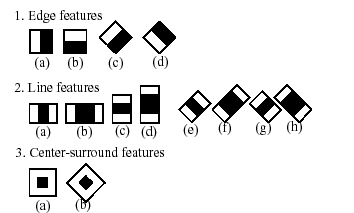
\includegraphics[width=0.5\textwidth]{pics/haarfeatures.png}

The feature used in a particular classifier is specified by its shape (1a, 2b etc.), position within the region of interest and the scale (this scale is not the same as the scale used at the detection stage, though these two scales are multiplied). For example, in the case of the third line feature (2c) the response is calculated as the difference between the sum of image pixels under the rectangle covering the whole feature (including the two white stripes and the black stripe in the middle) and the sum of the image pixels under the black stripe multiplied by 3 in order to compensate for the differences in the size of areas. The sums of pixel values over a rectangular regions are calculated rapidly using integral images (see below and the \cvCPyCross{Integral} description).

\ifPy
A simple demonstration of face detection, which draws a rectangle around each detected face:

\begin{lstlisting}

hc = cv.Load("haarcascade_frontalface_default.xml")
img = cv.LoadImage("faces.jpg", 0)
faces = cv.HaarDetectObjects(img, hc, cv.CreateMemStorage())
for (x,y,w,h),n in faces:
    cv.Rectangle(img, (x,y), (x+w,y+h), 255)
cv.SaveImage("faces_detected.jpg", img)

\end{lstlisting}

\fi

\ifC
To see the object detector at work, have a look at the HaarFaceDetect demo.

The following reference is for the detection part only. There
is a separate application called \texttt{haartraining} that can
train a cascade of boosted classifiers from a set of samples. See
\texttt{opencv/apps/haartraining} for details.

\cvclass{CvHaarFeature, CvHaarClassifier, CvHaarStageClassifier, CvHaarClassifierCascade}
\label{CvHaarFeature}
\label{CvHaarClassifier}
\label{CvHaarStageClassifier}
\label{CvHaarClassifierCascade}

Boosted Haar classifier structures.

\begin{lstlisting}
#define CV_HAAR_FEATURE_MAX  3

/* a haar feature consists of 2-3 rectangles with appropriate weights */
typedef struct CvHaarFeature
{
    int  tilted;  /* 0 means up-right feature, 1 means 45--rotated feature */

    /* 2-3 rectangles with weights of opposite signs and
       with absolute values inversely proportional to the areas of the 
       rectangles.  If rect[2].weight !=0, then
       the feature consists of 3 rectangles, otherwise it consists of 2 */
    struct
    {
        CvRect r;
        float weight;
    } rect[CV_HAAR_FEATURE_MAX];
}
CvHaarFeature;

/* a single tree classifier (stump in the simplest case) that returns the 
   response for the feature at the particular image location (i.e. pixel 
   sum over subrectangles of the window) and gives out a value depending 
   on the response */
typedef struct CvHaarClassifier
{
    int count;  /* number of nodes in the decision tree */

    /* these are "parallel" arrays. Every index \texttt{i}
       corresponds to a node of the decision tree (root has 0-th index).

       left[i] - index of the left child (or negated index if the 
         left child is a leaf)
       right[i] - index of the right child (or negated index if the 
          right child is a leaf)
       threshold[i] - branch threshold. if feature responce is <= threshold, 
                    left branch is chosen, otherwise right branch is chosen.
       alpha[i] - output value correponding to the leaf. */
    CvHaarFeature* haar_feature;
    float* threshold;
    int* left;
    int* right;
    float* alpha;
}
CvHaarClassifier;

/* a boosted battery of classifiers(=stage classifier):
   the stage classifier returns 1
   if the sum of the classifiers responses
   is greater than \texttt{threshold} and 0 otherwise */
typedef struct CvHaarStageClassifier
{
    int  count;  /* number of classifiers in the battery */
    float threshold; /* threshold for the boosted classifier */
    CvHaarClassifier* classifier; /* array of classifiers */

    /* these fields are used for organizing trees of stage classifiers,
       rather than just stright cascades */
    int next;
    int child;
    int parent;
}
CvHaarStageClassifier;

typedef struct CvHidHaarClassifierCascade CvHidHaarClassifierCascade;

/* cascade or tree of stage classifiers */
typedef struct CvHaarClassifierCascade
{
    int  flags; /* signature */
    int  count; /* number of stages */
    CvSize orig_window_size; /* original object size (the cascade is 
                            trained for) */

    /* these two parameters are set by cvSetImagesForHaarClassifierCascade */
    CvSize real_window_size; /* current object size */
    double scale; /* current scale */
    CvHaarStageClassifier* stage_classifier; /* array of stage classifiers */
    CvHidHaarClassifierCascade* hid_cascade; /* hidden optimized 
                        representation of the 
                        cascade, created by 
                cvSetImagesForHaarClassifierCascade */
}
CvHaarClassifierCascade;
\end{lstlisting}

All the structures are used for representing a cascaded of boosted Haar classifiers. The cascade has the following hierarchical structure:

\begin{verbatim}
    Cascade:
        Stage,,1,,:
            Classifier,,11,,:
                Feature,,11,,
            Classifier,,12,,:
                Feature,,12,,
            ...
        Stage,,2,,:
            Classifier,,21,,:
                Feature,,21,,
            ...
        ...
\end{verbatim}

The whole hierarchy can be constructed manually or loaded from a file or an embedded base using the function \cvCPyCross{LoadHaarClassifierCascade}.

\cvCPyFunc{LoadHaarClassifierCascade}
Loads a trained cascade classifier from a file or the classifier database embedded in OpenCV.

\cvdefC{
CvHaarClassifierCascade* cvLoadHaarClassifierCascade( \par const char* directory,\par CvSize orig\_window\_size );
}

\begin{description}
\cvarg{directory}{Name of the directory containing the description of a trained cascade classifier}
\cvarg{orig\_window\_size}{Original size of the objects the cascade has been trained on. Note that it is not stored in the cascade and therefore must be specified separately}
\end{description}

The function loads a trained cascade
of haar classifiers from a file or the classifier database embedded in
OpenCV. The base can be trained using the \texttt{haartraining} application
(see opencv/apps/haartraining for details).

\textbf{The function is obsolete}. Nowadays object detection classifiers are stored in XML or YAML files, rather than in directories. To load a cascade from a file, use the \cvCPyCross{Load} function.

\fi

\cvCPyFunc{HaarDetectObjects}
Detects objects in the image.

\ifC
\begin{lstlisting}
typedef struct CvAvgComp
{
    CvRect rect; /* bounding rectangle for the object (average rectangle of a group) */
    int neighbors; /* number of neighbor rectangles in the group */
}
CvAvgComp;
\end{lstlisting}
\fi

\cvdefC{
CvSeq* cvHaarDetectObjects( \par const CvArr* image,\par CvHaarClassifierCascade* cascade,\par CvMemStorage* storage,\par double scale\_factor=1.1,\par int min\_neighbors=3,\par int flags=0,\par CvSize min\_size=cvSize(0,\par0) );
}\cvdefPy{HaarDetectObjects(image,cascade,storage,scale\_factor=1.1,min\_neighbors=3,flags=0,min\_size=(0,0))-> detected\_objects}

\begin{description}
\cvarg{image}{Image to detect objects in}
\cvarg{cascade}{Haar classifier cascade in internal representation}
\cvarg{storage}{Memory storage to store the resultant sequence of the object candidate rectangles}
\cvarg{scale\_factor}{The factor by which the search window is scaled between the subsequent scans, 1.1 means increasing window by 10\% }
\cvarg{min\_neighbors}{Minimum number (minus 1) of neighbor rectangles that makes up an object. All the groups of a smaller number of rectangles than \texttt{min\_neighbors}-1 are rejected. If \texttt{min\_neighbors} is 0, the function does not any grouping at all and returns all the detected candidate rectangles, which may be useful if the user wants to apply a customized grouping procedure}
\cvarg{flags}{Mode of operation. Currently the only flag that may be specified is \texttt{CV\_HAAR\_DO\_CANNY\_PRUNING}. If it is set, the function uses Canny edge detector to reject some image regions that contain too few or too much edges and thus can not contain the searched object. The particular threshold values are tuned for face detection and in this case the pruning speeds up the processing}
\cvarg{min\_size}{Minimum window size. By default, it is set to the size of samples the classifier has been trained on ($\sim 20\times 20$ for face detection)}
\end{description}

The function finds rectangular regions in the given image that are likely to contain objects the cascade has been trained for and returns those regions as a sequence of rectangles. The function scans the image several times at different scales (see \cvCPyCross{SetImagesForHaarClassifierCascade}). Each time it considers overlapping regions in the image and applies the classifiers to the regions using \cvCPyCross{RunHaarClassifierCascade}. It may also apply some heuristics to reduce number of analyzed regions, such as Canny prunning. After it has proceeded and collected the candidate rectangles (regions that passed the classifier cascade), it groups them and returns a sequence of average rectangles for each large enough group. The default parameters (\texttt{scale\_factor} =1.1, \texttt{min\_neighbors} =3, \texttt{flags} =0) are tuned for accurate yet slow object detection. For a faster operation on real video images the settings are: \texttt{scale\_factor} =1.2, \texttt{min\_neighbors} =2, \texttt{flags} =\texttt{CV\_HAAR\_DO\_CANNY\_PRUNING}, \texttt{min\_size} =\textit{minimum possible face size} (for example, $\sim$ 1/4 to 1/16 of the image area in the case of video conferencing).

\ifPy
The function returns a list of tuples, \texttt{(rect, neighbors)}, where rect is a \cross{CvRect} specifying the object's extents
and neighbors is a number of neighbors.

\begin{lstlisting}
>>> import cv
>>> image = cv.LoadImageM("lena.jpg", cv.CV_LOAD_IMAGE_GRAYSCALE)
>>> cascade = cv.Load("../../data/haarcascades/haarcascade_frontalface_alt.xml")
>>> print cv.HaarDetectObjects(image, cascade, cv.CreateMemStorage(0), 1.2, 2, 0, (20, 20))
[((217, 203, 169, 169), 24)]
\end{lstlisting}
\fi

\ifC
% ===== Example. Using cascade of Haar classifiers to find objects (e.g. faces). =====
\begin{lstlisting}
#include "cv.h"
#include "highgui.h"

CvHaarClassifierCascade* load_object_detector( const char* cascade_path )
{
    return (CvHaarClassifierCascade*)cvLoad( cascade_path );
}

void detect_and_draw_objects( IplImage* image,
                              CvHaarClassifierCascade* cascade,
                              int do_pyramids )
{
    IplImage* small_image = image;
    CvMemStorage* storage = cvCreateMemStorage(0);
    CvSeq* faces;
    int i, scale = 1;

    /* if the flag is specified, down-scale the input image to get a
       performance boost w/o loosing quality (perhaps) */
    if( do_pyramids )
    {
        small_image = cvCreateImage( cvSize(image->width/2,image->height/2), IPL_DEPTH_8U, 3 );
        cvPyrDown( image, small_image, CV_GAUSSIAN_5x5 );
        scale = 2;
    }

    /* use the fastest variant */
    faces = cvHaarDetectObjects( small_image, cascade, storage, 1.2, 2, CV_HAAR_DO_CANNY_PRUNING );

    /* draw all the rectangles */
    for( i = 0; i < faces->total; i++ )
    {
        /* extract the rectanlges only */
        CvRect face_rect = *(CvRect*)cvGetSeqElem( faces, i );
        cvRectangle( image, cvPoint(face_rect.x*scale,face_rect.y*scale),
                     cvPoint((face_rect.x+face_rect.width)*scale,
                             (face_rect.y+face_rect.height)*scale),
                     CV_RGB(255,0,0), 3 );
    }

    if( small_image != image )
        cvReleaseImage( &small_image );
    cvReleaseMemStorage( &storage );
}

/* takes image filename and cascade path from the command line */
int main( int argc, char** argv )
{
    IplImage* image;
    if( argc==3 && (image = cvLoadImage( argv[1], 1 )) != 0 )
    {
        CvHaarClassifierCascade* cascade = load_object_detector(argv[2]);
        detect_and_draw_objects( image, cascade, 1 );
        cvNamedWindow( "test", 0 );
        cvShowImage( "test", image );
        cvWaitKey(0);
        cvReleaseHaarClassifierCascade( &cascade );
        cvReleaseImage( &image );
    }

    return 0;
}
\end{lstlisting}


\cvCPyFunc{SetImagesForHaarClassifierCascade}
Assigns images to the hidden cascade.

\cvdefC{
void cvSetImagesForHaarClassifierCascade( \par CvHaarClassifierCascade* cascade,\par const CvArr* sum,\par const CvArr* sqsum,\par const CvArr* tilted\_sum,\par double scale );
}

\begin{description}
\cvarg{cascade}{Hidden Haar classifier cascade, created by \cvCPyCross{CreateHidHaarClassifierCascade}}
\cvarg{sum}{Integral (sum) single-channel image of 32-bit integer format. This image as well as the two subsequent images are used for fast feature evaluation and brightness/contrast normalization. They all can be retrieved from input 8-bit or floating point single-channel image using the function \cvCPyCross{Integral}}
\cvarg{sqsum}{Square sum single-channel image of 64-bit floating-point format}
\cvarg{tilted\_sum}{Tilted sum single-channel image of 32-bit integer format}
\cvarg{scale}{Window scale for the cascade. If \texttt{scale} =1, the original window size is used (objects of that size are searched) - the same size as specified in \cvCPyCross{LoadHaarClassifierCascade} (24x24 in the case of \texttt{default\_face\_cascade}), if \texttt{scale} =2, a two times larger window is used (48x48 in the case of default face cascade). While this will speed-up search about four times, faces smaller than 48x48 cannot be detected}
\end{description}

The function assigns images and/or window scale to the hidden classifier cascade. If image pointers are NULL, the previously set images are used further (i.e. NULLs mean "do not change images"). Scale parameter has no such a "protection" value, but the previous value can be retrieved by the \cvCPyCross{GetHaarClassifierCascadeScale} function and reused again. The function is used to prepare cascade for detecting object of the particular size in the particular image. The function is called internally by \cvCPyCross{HaarDetectObjects}, but it can be called by the user if they are using the lower-level function \cvCPyCross{RunHaarClassifierCascade}.

\cvCPyFunc{ReleaseHaarClassifierCascade}
Releases the haar classifier cascade.

\cvdefC{
void cvReleaseHaarClassifierCascade( \par CvHaarClassifierCascade** cascade );
}

\begin{description}
\cvarg{cascade}{Double pointer to the released cascade. The pointer is cleared by the function}
\end{description}

The function deallocates the cascade that has been created manually or loaded using \cvCPyCross{LoadHaarClassifierCascade} or \cvCPyCross{Load}.

\cvCPyFunc{RunHaarClassifierCascade}
Runs a cascade of boosted classifiers at the given image location.

\cvdefC{
int cvRunHaarClassifierCascade( \par CvHaarClassifierCascade* cascade,\par CvPoint pt,\par int start\_stage=0 );
}

\begin{description}
\cvarg{cascade}{Haar classifier cascade}
\cvarg{pt}{Top-left corner of the analyzed region. Size of the region is a original window size scaled by the currenly set scale. The current window size may be retrieved using the \cvCPyCross{GetHaarClassifierCascadeWindowSize} function}
\cvarg{start\_stage}{Initial zero-based index of the cascade stage to start from. The function assumes that all the previous stages are passed. This feature is used internally by \cvCPyCross{HaarDetectObjects} for better processor cache utilization}
\end{description}

The function runs the Haar classifier
cascade at a single image location. Before using this function the
integral images and the appropriate scale (window size) should be set
using \cvCPyCross{SetImagesForHaarClassifierCascade}. The function returns
a positive value if the analyzed rectangle passed all the classifier stages
(it is a candidate) and a zero or negative value otherwise.

\fi

\fi

\ifCpp

\cvclass{FeatureEvaluator}
Base class for computing feature values in cascade classifiers.

\begin{lstlisting}
class CV_EXPORTS FeatureEvaluator
{
public:    
    enum { HAAR = 0, LBP = 1 }; // supported feature types 
    virtual ~FeatureEvaluator(); // destructor
    virtual bool read(const FileNode& node);
    virtual Ptr<FeatureEvaluator> clone() const;
    virtual int getFeatureType() const;
    
    virtual bool setImage(const Mat& img, Size origWinSize);
    virtual bool setWindow(Point p);

    virtual double calcOrd(int featureIdx) const;
    virtual int calcCat(int featureIdx) const;

    static Ptr<FeatureEvaluator> create(int type);
};
\end{lstlisting}

\cvCppFunc{FeatureEvaluator::read}
Reads parameters of the features from a FileStorage node.

\cvdefCpp{
bool FeatureEvaluator::read(const FileNode\& node);
}

\begin{description}
\cvarg{node}{File node from which the feature parameters are read.}
\end{description}

\cvCppFunc{FeatureEvaluator::clone}
Returns a full copy of the feature evaluator.

\cvdefCpp{
Ptr<FeatureEvaluator> FeatureEvaluator::clone() const;
}

\cvCppFunc{FeatureEvaluator::getFeatureType}
Returns the feature type (HAAR or LBP for now).

\cvdefCpp{
int FeatureEvaluator::getFeatureType() const;
}

\cvCppFunc{FeatureEvaluator::setImage}
Sets the image in which to compute the features.

\cvdefCpp{
bool FeatureEvaluator::setImage(const Mat\& img, Size origWinSize);
}

\begin{description}
\cvarg{img}{Matrix of type  \texttt{CV\_8UC1} containing the image in which to compute the features.}
\cvarg{origWinSize}{Size of training images.}
\end{description}

\cvCppFunc{FeatureEvaluator::setWindow}
Sets window in the current image in which the features will be computed (called by \cvCppCross{CascadeClassifier::runAt}).

\cvdefCpp{
bool FeatureEvaluator::setWindow(Point p); 
}

\begin{description}
\cvarg{p}{The upper left point of window in which the features will be computed. Size of the window is equal to size of training images.}
\end{description}

\cvCppFunc{FeatureEvaluator::calcOrd}
Computes value of an ordered (numerical) feature.

\cvdefCpp{
double FeatureEvaluator::calcOrd(int featureIdx) const;
}

\begin{description}
\cvarg{featureIdx}{Index of feature whose value will be computed.}
\end{description}
Returns computed value of ordered feature.

\cvCppFunc{FeatureEvaluator::calcCat}
Computes value of a categorical feature.

\cvdefCpp{
int FeatureEvaluator::calcCat(int featureIdx) const;
}

\begin{description}
\cvarg{featureIdx}{Index of feature whose value will be computed.}
\end{description}
Returns computed label of categorical feature, i.e. value from [0,... (number of categories - 1)].

\cvCppFunc{FeatureEvaluator::create}
Constructs feature evaluator.

\cvdefCpp{
static Ptr<FeatureEvaluator> FeatureEvaluator::create(int type);
}

\begin{description}
\cvarg{type}{Type of features evaluated by cascade (HAAR or LBP for now).}
\end{description}

\cvclass{CascadeClassifier}
The cascade classifier class for object detection.

\begin{lstlisting}
class CascadeClassifier
{
public:
	// structure for storing tree node
    struct CV_EXPORTS DTreeNode 
    {
        int featureIdx; // feature index on which is a split
        float threshold; // split threshold of ordered features only
        int left; // left child index in the tree nodes array
        int right; // right child index in the tree nodes array
    };
    
    // structure for storing desision tree
    struct CV_EXPORTS DTree 
    {
        int nodeCount; // nodes count
    };
    
    // structure for storing cascade stage (BOOST only for now)
    struct CV_EXPORTS Stage
    {
        int first; // first tree index in tree array
        int ntrees; // number of trees
        float threshold; // treshold of stage sum
    };
    
    enum { BOOST = 0 }; // supported stage types
    
    // mode of detection (see parameter flags in function HaarDetectObjects)
    enum { DO_CANNY_PRUNING = CV_HAAR_DO_CANNY_PRUNING,
           SCALE_IMAGE = CV_HAAR_SCALE_IMAGE,
           FIND_BIGGEST_OBJECT = CV_HAAR_FIND_BIGGEST_OBJECT,
           DO_ROUGH_SEARCH = CV_HAAR_DO_ROUGH_SEARCH }; 

    CascadeClassifier(); // default constructor
    CascadeClassifier(const string& filename);
    ~CascadeClassifier(); // destructor
    
    bool empty() const;
    bool load(const string& filename);
    bool read(const FileNode& node);

    void detectMultiScale( const Mat& image, vector<Rect>& objects, 
                           double scaleFactor=1.1, int minNeighbors=3, 
						   int flags=0, Size minSize=Size());
    
    bool setImage( Ptr<FeatureEvaluator>&, const Mat& );
    int runAt( Ptr<FeatureEvaluator>&, Point );

    bool is_stump_based; // true, if the trees are stumps

    int stageType; // stage type (BOOST only for now)
    int featureType; // feature type (HAAR or LBP for now)
    int ncategories; // number of categories (for categorical features only) 
    Size origWinSize; // size of training images
    
    vector<Stage> stages; // vector of stages (BOOST for now)
    vector<DTree> classifiers; // vector of decision trees
    vector<DTreeNode> nodes; // vector of tree nodes
    vector<float> leaves; // vector of leaf values
    vector<int> subsets; // subsets of split by categorical feature

    Ptr<FeatureEvaluator> feval; // pointer to feature evaluator
    Ptr<CvHaarClassifierCascade> oldCascade; // pointer to old cascade
};
\end{lstlisting}

\cvCppFunc{CascadeClassifier::CascadeClassifier}
Loads the classifier from file.

\cvdefCpp{
CascadeClassifier::CascadeClassifier(const string\& filename);
}

\begin{description}
\cvarg{filename}{Name of file from which classifier will be load.}
\end{description}

\cvCppFunc{CascadeClassifier::empty}
Checks if the classifier has been loaded or not.

\cvdefCpp{
bool CascadeClassifier::empty() const;
}

\cvCppFunc{CascadeClassifier::load}
Loads the classifier from file. The previous content is destroyed.

\cvdefCpp{
bool CascadeClassifier::load(const string\& filename);
}

\begin{description}
\cvarg{filename}{Name of file from which classifier will be load. File may contain as old haar classifier (trained by haartraining application) or new cascade classifier (trained traincascade application).}
\end{description}

\cvCppFunc{CascadeClassifier::read}
Reads the classifier from a FileStorage node. File may contain a new cascade classifier (trained traincascade application) only.

\cvdefCpp{
bool CascadeClassifier::read(const FileNode\& node);
}

\cvCppFunc{CascadeClassifier::detectMultiScale}
Detects objects of different sizes in the input image. The detected objects are returned as a list of rectangles.

\cvdefCpp{
void CascadeClassifier::detectMultiScale( const Mat\& image,
                           vector<Rect>\& objects,
                           double scaleFactor=1.1,
                           int minNeighbors=3, int flags=0,
                           Size minSize=Size());
}

\begin{description}
\cvarg{image}{Matrix of type  \texttt{CV\_8U} containing the image in which to detect objects.}
\cvarg{objects}{Vector of rectangles such that each rectangle contains the detected object.}
\cvarg{scaleFactor}{Specifies how much the image size is reduced at each image scale.}
\cvarg{minNeighbors}{Speficifes how many neighbors should each candiate rectangle have to retain it.}
\cvarg{flags}{This parameter is not used for new cascade and have the same meaning for old cascade as in function cvHaarDetectObjects.}
\cvarg{minSize}{The minimum possible object size. Objects smaller than that are ignored.}
\end{description}

\cvCppFunc{CascadeClassifier::setImage}
Sets the image for detection (called by detectMultiScale at each image level).

\cvdefCpp{
bool CascadeClassifier::setImage( Ptr<FeatureEvaluator>\& feval, const Mat\& image );
}

\begin{description}
\cvarg{feval}{Pointer to feature evaluator which is used for computing features.}
\cvarg{image}{Matrix of type  \texttt{CV\_8UC1} containing the image in which to compute the features.}
\end{description}

\cvCppFunc{CascadeClassifier::runAt}
Runs the detector at the specified point (the image that the detector is working with should be set by setImage).

\cvdefCpp{
int CascadeClassifier::runAt( Ptr<FeatureEvaluator>\& feval, Point pt );
}

\begin{description}
\cvarg{feval}{Feature evaluator which is used for computing features.}
\cvarg{pt}{The upper left point of window in which the features will be computed. Size of the window is equal to size of training images.}
\end{description}
Returns:
1 - if cascade classifier detects object in the given location.
-si - otherwise. si is an index of stage which first predicted that given window is a background image.

\cvCppFunc{groupRectangles}
Groups the object candidate rectangles

\cvdefCpp{void groupRectangles(vector<Rect>\& rectList,\par
                     int groupThreshold, double eps=0.2);}
\begin{description}
\cvarg{rectList}{The input/output vector of rectangles. On output there will be retained and grouped rectangles}
\cvarg{groupThreshold}{The minimum possible number of rectangles, minus 1, in a group of rectangles to retain it.}
\cvarg{eps}{The relative difference between sides of the rectangles to merge them into a group}
\end{description}

The function is a wrapper for a generic function \cvCppCross{partition}. It clusters all the input rectangles using the rectangle equivalence criteria, that combines rectangles that have similar sizes and similar locations (the similarity is defined by \texttt{eps}). When \texttt{eps=0}, no clustering is done at all. If $\texttt{eps}\rightarrow +\inf$, all the rectangles will be put in one cluster. Then, the small clusters, containing less than or equal to \texttt{groupThreshold} rectangles, will be rejected. In each other cluster the average rectangle will be computed and put into the output rectangle list.  
\fi
